	\section{Второй билет. Основные классы биологический молекул, ДНК, генетический код}
	Кто хочет подробней открывайте Альбертса с 59ой страницы. Тут только малая часть того что там есть
	\subsection{Основыне классы биологический молекул}
	\paragraph{Углеводны} Они же сахара. Содержат альдегидную группу $\ce{C=O}$ А так же несколько гидроксильных групп $\ce{O - H}$. Простейшим примером является глюкоза $\ce{C6H12O6}$, которая частный случай моносахарида $\ce{(CH2O)_n}$ где $n$ любое натуральное число. Углеводы могут существовать либо в форме кольца, либо
в виде открытой цепи. К одному кольцо может через атом углерода альдегидной группы присоединиться еще одно кольцо, образуя дисахарид. Например мальтоза (см картинку ниже). Можно образовывать еще большие последовательности, называются полисахаридами.
	\begin{figure}[H]
		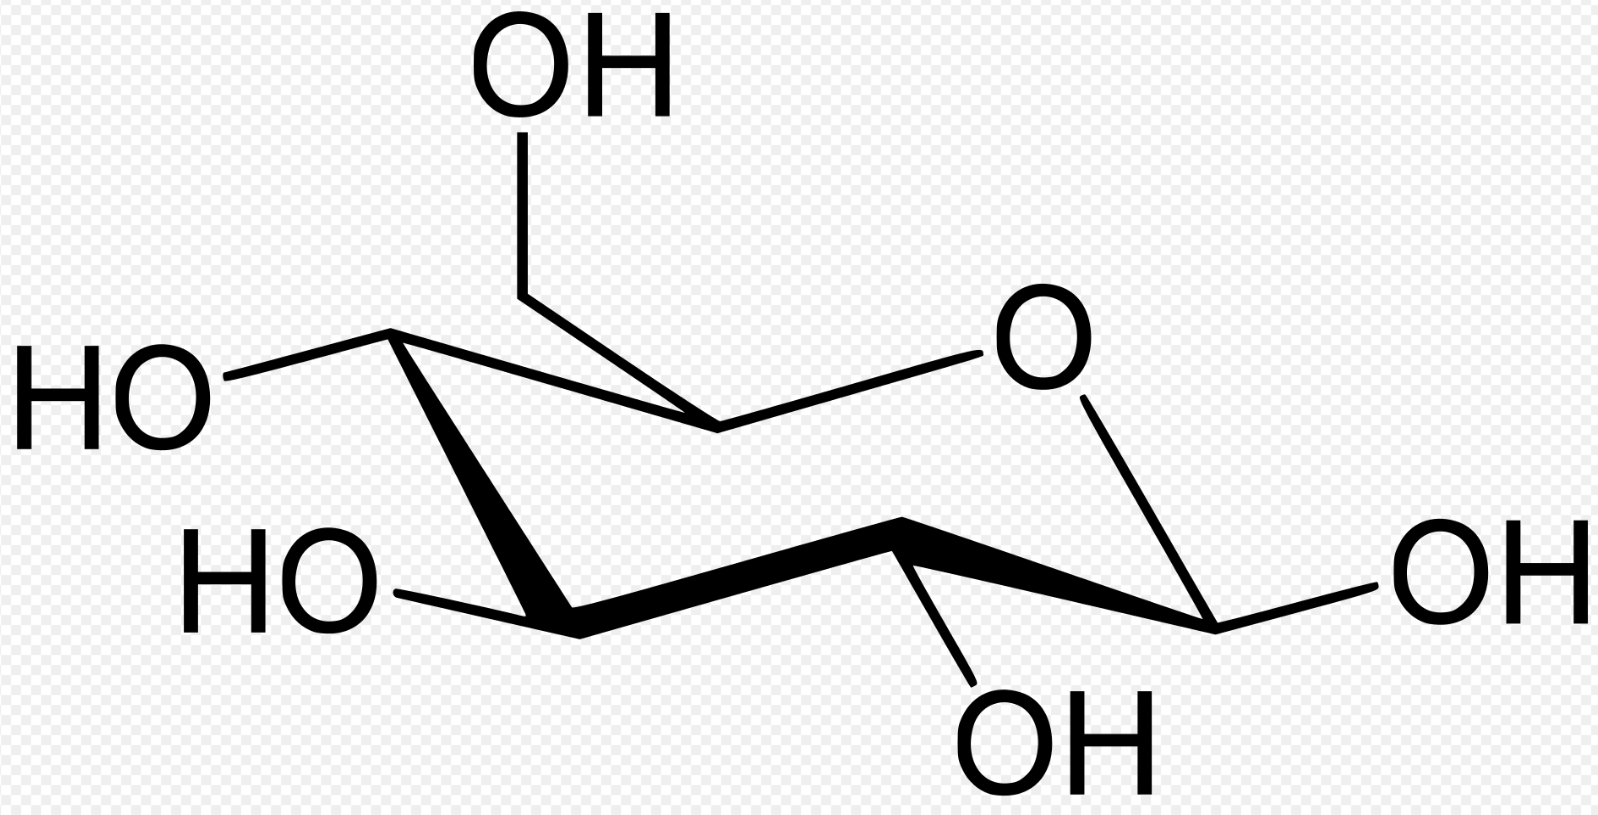
\includegraphics[scale = 0.2]{2glu}\\
		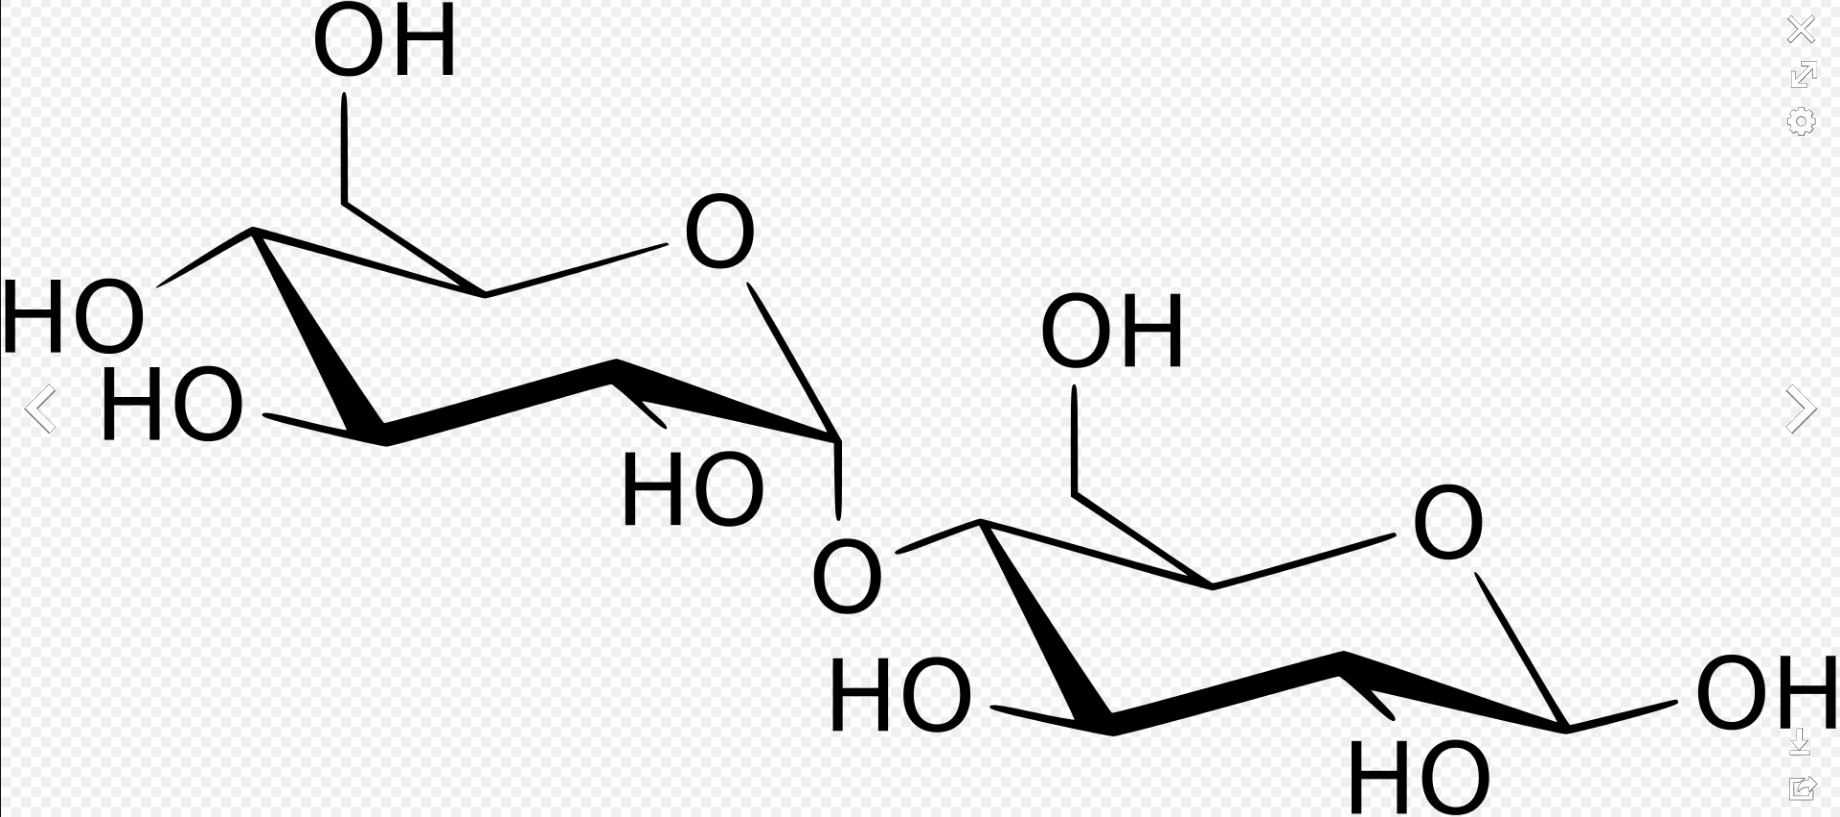
\includegraphics[scale = 0.2]{2mal}
		\caption{Глюкоза и мальтоза}
	\end{figure}
Глюкоза служит главным источником энергии во многих клетках. В результате последовательного ряда реакций окисления эта гексоза превращается в различные производные Сахаров с меньшей длиной цепи и в конечном итоге распадается до $\ce{CO2}$ и $\ce{H2O}$. В ходе распада глюкозы высвобождается энергия и генерируется восстановительная способность, без чего невозможно протекание
биосинтетических реакций. Высвобождающаяся энергия и генерируемая восстановительная сила запасаются в форме двух важнейших соединений -
АТР и NADH. Так же из углеводов состоит важный внеклеточный структурный материал (например целлюлоза) 
	\paragraph{Липиды} они же жиры. У них обычно имеются две различные части: длинная углеводородная цепь,
	которая имеет гидрофобный характер (водонерастворима) и химически мало активна, и карбоксильная группа, ионизирующаяся в растворе, крайне
	гидрофильная (водорастворимая) и легко образующая эфиры и амиды.\\
	Жирные кислоты являются ценным источником энергии, поскольку их
	расщепление сопровождается образованием такого количества АТР, которое в два раза
	превышает образование АТР при расщеплении такого же количества (по массе)
	глюкозы. Жирные кислоты запасаются в цитоплазме многих клеток в виде капелек
	триацилглицеролов (триглицеридов). Молекулы триацилглицеролов состоят из трех
	цепей жирных кислот, каждая из которых присоединена к молекуле глицерола  именно так устроены животные жиры, с которыми мы имеем дело в
	повседневной жизни.\\
	Но самая важная функция жирных кислот - участие в построении клеточных
	мембран. Эти тонкие плотные пленки, которыми одеты все клетки и внутриклеточные
	органеллы, состоят главным образом из фосфолипидов
	\begin{figure}[H]
		\centering
		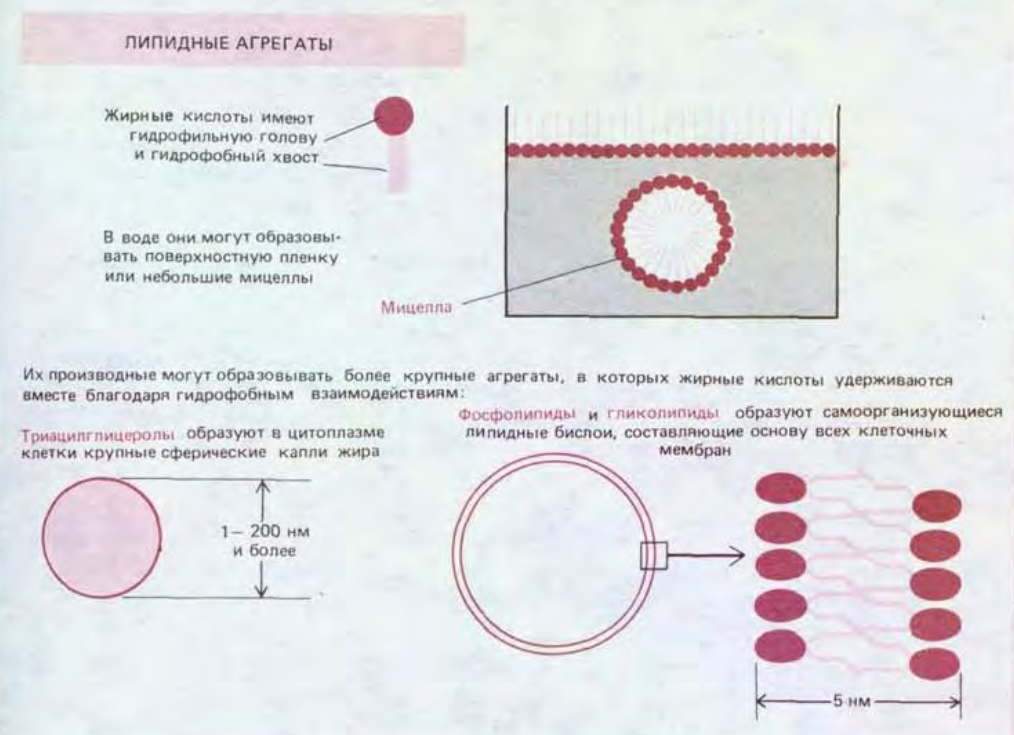
\includegraphics[scale=0.3]{2lipid}
	\end{figure}
	\paragraph{Аминокислоты} органические вещества которые состоят из аминогруппы и карбоксильной круппы
	\begin{figure}[H]
		\centering
		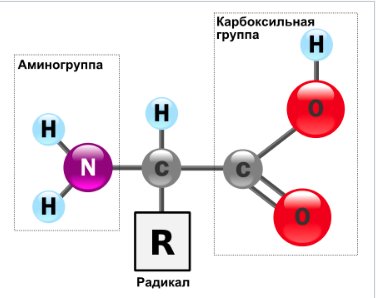
\includegraphics[scale= 0.7]{2amin}
	\end{figure}
Аминокислоты служат строительными блоками при синтезе белков
- длинных линейных полимеров аминокислот, соединенных «хвост к голове» при
помощи пептидной связи между карбоксильной группой одной аминокислоты и
аминогруппой другой. В белках встречается обычно 20 аминокислот с
разными радикалами. Одни и те
же 20 аминокислот неоднократно повторяются во всех белках, в том числе в белках
бактериального, животного и растительного происхождения.
	\paragraph{Нуклеотиды} Нуклеотиды являются сложными эфирами нуклеозидов и фосфорных кислот.
	\begin{figure}[H]
		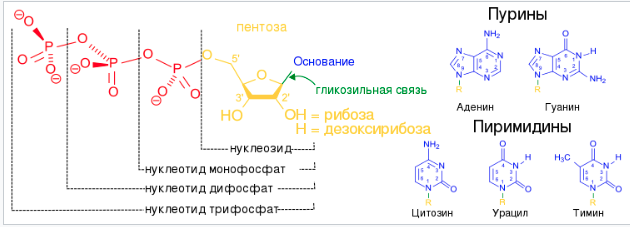
\includegraphics[scale = 0.7]{2nucle}
	\end{figure}
	Цитозин (С), тимин (Т) и урацил (U)
	называются пиримидиновыми основаниями, так как они представляют собой простые производные шестичленного пиримидинового кольца;
	гуанин (G) и аденин (А) - пуриновые основания, второе пятичленное кольцо которых сконденсировано с шестичленным циклом\\
	Нуклеотиды могут выступать в качестве переносчиков энергии. При этом трифосфатный эфир аденина АТР (рис. 2-9) гораздо чаще, чем
	другие нуклеотиды, участвует в переносе энергии между сотнями индивидуальных внутриклеточных реакций. Энергия высвобождающаяся в результате гидролиза АТФ может использоваться в любой другой реакции которая проходит с поглощением энергии.
	\begin{figure}[H]
		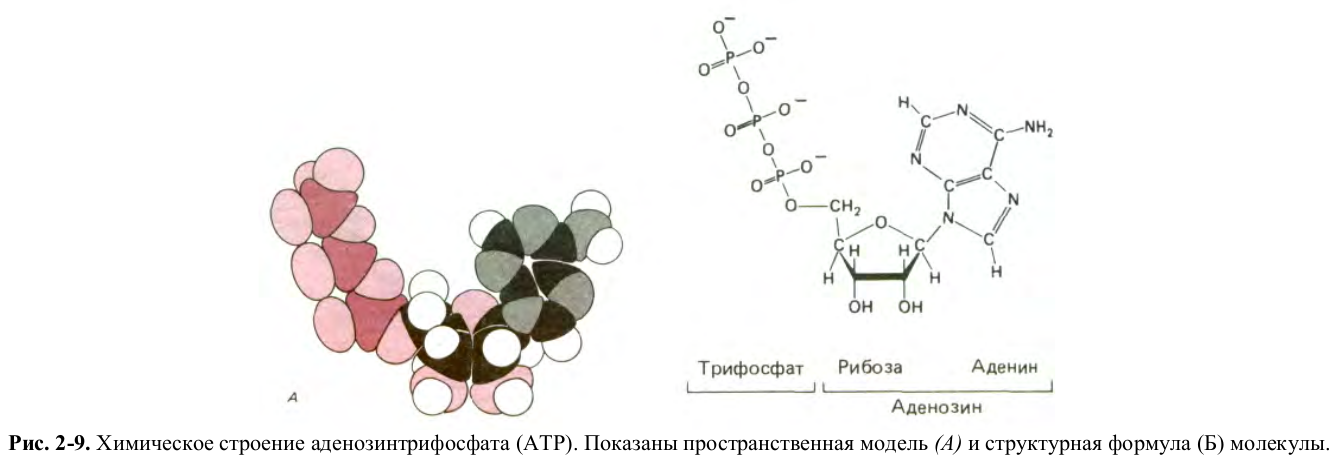
\includegraphics[scale=0.4]{2atf}
	\end{figure}
	Другие производные
	нуклеотидов служат переносчиками отдельных химических групп, таких, как атомы водорода или остатки Сахаров, с одной молекулы на другую. Кроме того, циклическое фосфорилированное производное аденинациклический AMP (cAMP) -служит универсальным внутриклеточным сигналом и
	регулирует скорость множества различных внутриклеточных реакций. \\
	
	Нуклеотиды служат
	строительными блоками для синтеза нуклеиновых кислот - длинных полимеров, в которых нуклеотидные субъединицы соединяются между собой
	ковалентной связью, образуя фосфорный эфир между 3'-гидроксильной группой остатка сахара одного нуклеотида и 5'-фосфатной группой. Нуклеиновые кислоты, сахар которых представлен рибозой, называются рибонуклеиновыми кислотами или \textbf{РНК}; они
	содержат основания A, U, G и С. Те нуклеиновые кислоты, в состав которых входит дезоксирибоза (в ней гидроксильная группа при С-2 рибозы
	замещена на атом водорода), называются дезоксирибонуклеиновыми кислотами или \textbf{ДНК}; они содержат основания А, Т, G и С. Способность к спариванию G c C и A c T лежит в основе механизмов хранения и передачи наследственно информации.
	
	\subsection{Формы ДНК}
	Наиболее распространой является В-форма. В этой форме находится основная часть ДНК в клетках. При такой организации плоскости азотистых оснований практически перпендикулярны оси двойной спирали, и каждая пара повёрнута относительно предыдущих на $36^\circ$. На один виток спирали приходится примерно 10 нуклеотидных пар (9,7 и 10,6 в различных кристаллах)(2), а длина составляет 3,4 нм.
	\begin{figure}[H]
		\centering
		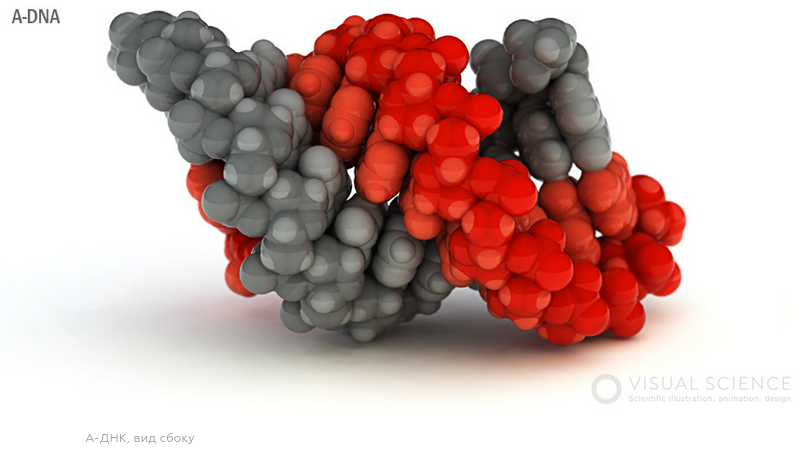
\includegraphics[scale = 0.5]{2adnk}
	\end{figure}
Существенным отличием А-формы от В-формы является то, что в А-форме пары оснований сдвинуты к периферии спирали почти на половину её радиуса, в результате чего пространство вдоль оси оказывается пустым. Большая бороздка при этом становится глубже и уже, а малая бороздка оказывается шире и более плоской
	\begin{figure}[H]
		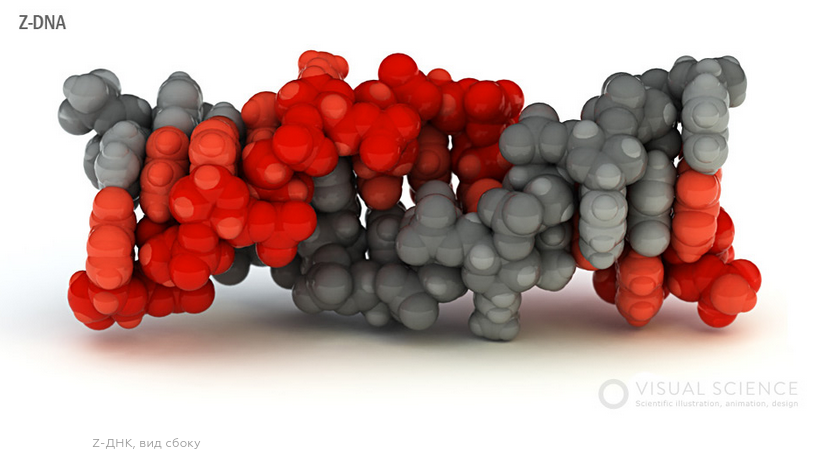
\includegraphics[scale=0.6]{2zdnk}
	\end{figure} 
Z форма представляет собой левозакрученную спираль с длиной витка 4,4 нм, на который приходится 12 нуклеотидных пар.
		\subsection{Отличие эукариот от прокариот}
		Прокариоты не имеют оформленного ядра. Их хромосомы имеют кольцевую форму. А гены объеденены в опероны.
		Эукариотические клетки по определению и в отличие от прокариотических имеют ядро (по гречески «карион»). Ядро, в котором
		находится большая часть клеточной ДНК, ограничено двойной мембраной. 
	
	\subsection{Генетический код}
	\textbf{Генетичесий код - совокупность правил, согласно которым в живых клетках последовательность нуклеотидов (ген и мРНК) переводится в последовательность аминокислот (белок).}\\
	Ген - участок днк определяющий определенную последовательность аминокислот.\\
	Аллели - различные формы одного и того же гена, расположенные в одинаковых участках (локусах) гомологичных хромосом, определяют направление развития конкретного признака
	
	\subsection{Митоз и мейоз}
	Мейоз (редукционное деление клетки) — деление, в процессе которого из одной диплоидной клетки получаются 4 гаплоидные клетки.
	\begin{figure}[H]
		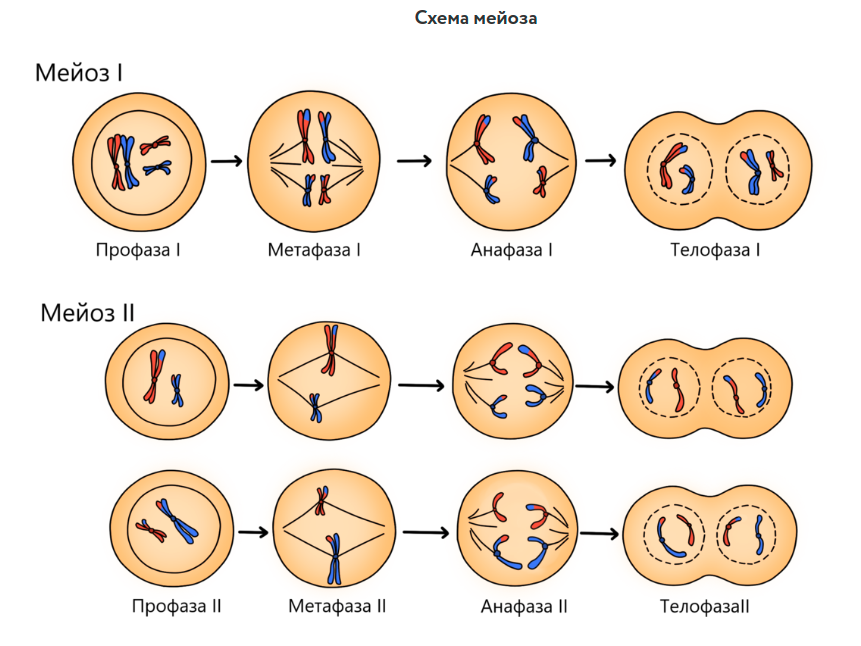
\includegraphics[scale=0.5]{2mi}
	\end{figure}
Мейоз у животных наблюдается при формировании гамет (гаметогенезе). Мейоз у растений и грибов, как правило, происходит при образовании гаплоидных спор. У различных одноклеточных эукариот мейоз может наблюдаться на разных стадиях жизненного цикла. Для восстановления диплоидности в цикле всегда необходимо слияние гаплоидных клеток (оплодотворение).\\
Мейоз состоит из двух делений. Первое из них является собственно редукционным, то есть именно в ходе первого деления уменьшается плоидность клетки. Причиной этого служит расхождение гомологичных хромосом («материнской» и «отцовской») по двум разным дочерним клеткам. Второе деление аналогично митозу и называется эквационным (то есть «равным»). Плоидность в результате второго деления не меняется. В ходе этого деления, как и при митозе, расходятся сестринские хроматиды (копии ДНК). Между двумя делениями мейоза отсутствует репликация ДНК (так как «цель» мейоза — уменьшить плоидность клетки, увеличивать количество ДНК здесь незачем).\\
В профазе I деления мейоза происходит важнейший процесс, относящийся к генетической рекомбинации — кроссинговер, то есть обмен участками гомологичных хромосом.\\

	\textbf{Митоз} - непрямое деление клетки, наиболее распространённый способ репродукции эукариотических клеток. Биологическое значение митоза состоит в строго одинаковом распределении хромосом между дочерними ядрами, что обеспечивает образование генетически идентичных дочерних клеток и сохраняет преемственность в ряду клеточных поколений. \textbf{Митоз лежит в основе бесполого размножения, от отличие от мейоза.}
	\newpage